% Dossier de synthèse
% Version 1.0

% Historique des versions
% 23/01/08 1.0 Création et remplissage (Mikado)

\documentclass[a4paper, 11pt, draft]{article}

\usepackage[utf8]{inputenc} % Texte en utf-8
\usepackage{aeguill}
\usepackage[francais]{babel} % Typographie française
\usepackage[pdftex, hypertexnames=false, colorlinks=true, final]{hyperref}
\usepackage[final]{graphicx}
\usepackage{url} % Gestion des URLs
\usepackage{geometry}
\usepackage{fancyhdr}

% Marges à gauche et à droite de 3cm
\geometry{margin=3cm}

% Utilisation des headers et footers personnalisés de fancyhdr
\pagestyle{fancy}

% Images dans le dossier ./images/
\graphicspath{{./images/}}

% Gestion des métadonnées étranges à rendre visibles au rendu
\newcommand\docname{SYNv1.0}
\newcommand\docauthor{Fabrice GABOLDE}
\newcommand\docstatus{LIVRABLE} % EN COURS, ATTENTE, VALIDE ou LIVRABLE

% Format de citation de références standard, marche avec quasiment tout
\newcommand\fullref[1]{\ref{#1}, page \pageref{#1}}

% En-têtes et pieds de page
\lhead{\docname}
\rhead{}
\lfoot{Auteur : H4213}
\cfoot{}
\rfoot{\thepage}

% Titre du document maître
\title{\textbf{COPEVUE}\\
\rule{\textwidth}{1pt}{}\\
\Huge{\textsc{Dossier de synthèse}}}
\author{\docauthor{} (H4213)}
\date{\docname{} --- \today{} (\docstatus{})}

\begin{document}

\maketitle

\tableofcontents

\section{Introduction}

\subsection*{Document \docname{}}

Auteur : \docauthor{}

Etat : \docstatus{}

\subsection{Présentation du projet}

Il existe aujourd'hui de nombreux sites isolés et/ou difficiles d'accès qui nécessitent une surveillance et parfois des actions à distance. Ces sites se situent dans des espaces très différents tels que les citernes placées dans les forêts escarpées du pourtour méditerranéen, les réservoirs utilisés pour l'autonomie des chantiers dans le grand Nord mais aussi les personnes âgées qui se retrouvent souvent isolées.

Actuellement tous les contrôles et actions sont réalisés par un opérateur qui doit se déplacer sur le site. Il n'y a donc que très peu de réactivité, on ne peut pas avoir un suivi fin des évolutions et des problèmes graves (par exemple la fuite d'un réservoir) ne peuvent pas être traités rapidement.

\paragraph{Etude COPEVUE}
L'objet de l'étude est la mise en place d'un système générique de surveillance et d'action à distance sur des sites isolés. Le système devra être évolutif, autonome et fiable.

\subsection{Présentation du document}

Ce document (Dossier de synthèse) présente les principaux choix et l'élaboration de la solution de l'étude COPEVUE, ainsi que les modifications entraînées par l'arrivée d'un nouveau système.

\subsubsection{Objectifs}

Voici les objectifs de ce document :
\begin{itemize}
\item Présentation de la solution proposée
\item Description de la mise en place du système
\end{itemize}

\subsection{Documents applicables et de référence}

\subsubsection{Documents applicables}

\begin{itemize}
\item Dossier de gestion de la documentation (DGD)
\end{itemize}

\subsubsection{Documents de référence}

Aucun.

\section{Présentation de la solution proposée}

\subsection{Architecture}

Les données récupérées des capteurs, ainsi que les données relatives au fonctionnement global du système (traçabilité, etc.) seront centralisées sur un serveur. Les postes de gestion fixes et les systèmes mobiles pourront y accéder, soit par des liaisons filaires, soit par un système de communication sans fil longue distance. Les sites isolés pourront ainsi communiquer avec le reste du système par les mêmes canaux longue distance.

Voir le schéma de l'architecture générale, en figure \fullref{figure:schema_archi_generale}.

\subsection{Fonctionnement général}

\subsubsection{Connaissance de l'état du site sur place}

Les intervenants disposeront d'un ordinateur portable ou d'un PDA, capable d'établir une liaison à distance (via la technologie GSM) comme filaire (port série ou USB). L'utilisation de deux modes possibles de liaison assure une connexion quelle que soit la défaillance.

\subsubsection{Connaissance de l'état du site à distance}
\label{subs:connaissance_etat_distance}

L'utilisation de la technologie GSM entraînera la création d'un réseau alternatif de communication et mènera par conséquent à la pose de nouvelles antennes. Des accords avec les opérateurs de téléphonie mobile implémentés dans le pays ainsi que des subventions de la part de l'Union Européenne seraient une possibilité. Ces accords permettraient à l'opérateur d'étendre sa couverture ; en contrepartie il serait capable de fournir une communication avec le site distant.

\subsubsection{Surveillance de l'état du site à distance}

Le transfert des informations recueillies par les systèmes de capteurs peut se faire sur le même réseau que celui utilisé pour la \emph{Connaissance de l'état du site à distance} (voir \fullref{subs:connaissance_etat_distance}). Toutes les anomalies détectées qui nécessitent une intervention humaine peuvent être envoyées aux administrateurs par les voies usuelles (e-mails, SMS, etc.).

\subsubsection{Configuration du site à distance}

Le protocole SSH permet d'accéder à un terminal distant via une liaison sécurisée. La configuration du site à distance pourra donc se faire exactement comme si on y avait accès sur place (opérations physiques mises à part).

\subsubsection{Fiabilité des données}

Dans tous les systèmes critiques, on procède à un triplement des capteurs de manière à pouvoir déceler avec une quasi certitude les défaillances des capteurs. L'augmentation du nombre d'interventions de maintenance que cela induit est compensée par la flexibilité gagnée dans les délais de réparation du système.

\subsubsection{Fiabilité du transfert des données}

Les réseaux GSM permettent de transférer des données numériques avec une fiabilité déjà excellente. Pour améliorer encore la fiabilité, une couche logicielle de vérification d'intégrité pourra être ajoutée. Il faut noter que la plupart des données n'exigent pas un transfert immédiat, on a donc une certaine souplesse sur les contraintes temporelles.

\subsubsection{Localisation géographique}

Le systeme central aura accès à la localisation géographique exacte et précise de chaque entité du système à l'aide de la technologie GPS qui est éprouvée, fiable, de précision suffisante pour notre utilisation et qui couvre la totalité du globe -- en particulier les sites isolés et les éléments mobiles.

\subsubsection{Traçabilité des opérations}

En phase de fonctionnement normal, les informations envoyées par chaque site sont immédiatement stockées sur le serveur central avant leur traitement. On enregistre chaque donnée avec ses méta-informations -- site de provenance, date, etc. Ces données sont préservées pendant une durée de quatre ans, considérant des contraintes légales et un besoin d'analyse statistique. Elles seront dupliquées pour éviter les pertes involontaires.
En plus des données des capteurs, en enregistrera l'historique des opérations de chaque contrôleur de capteur, pour chaque site. La fréquence des relevés sera fonction des capteurs, elle dépendra de la criticité de l'élément à surveiller, mais restera configurable.
Dans un souci de portabilité, le format de sauvegarde sera le texte brut.

\subsubsection{Autonomie énergétique des sites}

Les sites seront fournis en énergie par des accumulateurs longue durée non rechargeables. Dans les cas où les sites sont difficiles d'accès mais proposent une source énergétique facilement exploitable, ou pour des sites nécessitant un apport d'énergie important, on pourra utiliser les énergies renouvelables disponibles à proximité (s'agissant de la Norvège : photovoltaïque, éolienne et hydroélectrique), couplées à une batterie rechargeable.
% Mikado : revoir définition "accumulateur" : rechargeable ?

\subsubsection{Fiabilité, stabilité et reprise sur panne}

Dans le cas d'informations critiques, on prévoit de tripler les liaisons entre le système de pilotage informatique, les capteurs et les actionneurs. De même, on prendra en compte, lors de la conception de la solution, une possible reprise sur panne du système. Celle-ci peut être automatique -- si le système informatique local le décide -- pilotée à distance, ou planifiée.

\subsection{Apports de la solution proposée}

\subsubsection{Réactivité}

La solution que nous proposons permettra de réduire grandement le délai de transmission de l'information. Par rapport à l'existant, où tous les contrôles et toutes les actions sont effectués par un opérateur qui se rend en personne sur le site distant, l'automatisation du rapport des capteurs permettra une réactivité accrue. Une flexibilité au niveau de la fréquence de mise à jour sera également possible, pour permettre de suivre certaines données en quasi-temps réel, et avoir un rapport seulement toutes les 24h pour d'autres.
Les seuls déplacements physiques d'opérateurs requis devraient être ceux qui ne sont pas autrement automatisables : contrôles de routines de l'état du matériel, réparations mécaniques, etc.

\subsubsection{Continuité de service}

% Mikado : traduire failsafe correctement...
La garantie de fiabilité et stabilité que notre solution apporte, tant via le matériel rendu sûr par la multiplication des doublons que par le logiciel permettant un transfert des données sécurisé et fiable, assure une continuité de service la moins interrompue possible. En cas de problème, une reprise sur panne automatique pourra être assurée sur la plupart des cas. Ceci devrait réduire d'autant la nécessité des déplacements physiques mentionnés plus haut.

\subsubsection{Optimisation des coûts}

L'optimisation des déplacements, la fiabilité globale du système et l'amélioration globale du fonctionnement du système ainsi que de la présentation des données sont autant d'élements qui permettent d'assurer une réduction des coûts de fonctionnement, une fois la solution mise en place.

\section{Mise en place du système}

\subsection{Serveur et logiciel local}

Le premier élément à mettre en place est le système local. On installera donc le serveur central ainsi que les postes de gestion locaux reliés par liaison filaire. Ceci est une tâche d'administration classique et ne devrait donc pas prendre beaucoup de temps -- même en considérant le temps que peut prendre le remplacement de postes de travail pour les utilisateurs. Le développement du logiciel du serveur et des postes de gestion prendra nettement plus de temps (environ un an et demi : aucune estimation précise n'est disponible pour l'instant).

\subsection{Logiciel de l'intervenant}

Le logiciel de l'intervenant passera par le modèle de déploiement suivant :
\begin{description}
\item[6 mois] Développement et tests unitaires
\item[3 mois] Tests en simulation, tests d'intégration
\item[2 mois] Tests avec matériel, retour d'expérience
\item[3 mois] Finalisation, éventuellement reprise
\end{description}

\subsection{Logiciel embarqué}

Le logiciel embarqué passera par un modèle de déploiement similaire, pour lequel nous n'avons pas encore de valeurs de durée. Cependant, l'architecture plus modulaire du logiciel embarqué imposera une durée plus longue pour les tests unitaires et les tests d'intégration.

\subsection{Formation des utilisateurs}

La formation des utilisateurs pourra commencer dès la mise en place des postes de gestion locaux. On pourra éventuellement simuler le fonctionnement du système avec un ou plusieurs faux sites isolés comportant la batterie usuelle de capteurs. Ceci permettra aux administrateurs et aux utilisateurs de se familiariser avec le système.

\subsection{Installation du GSM}

En parallèle avec la mise en place du serveur et la formation des utilisateurs, on mettra en place le système GSM et négociera les contrats avec l'entreprise de télécommunications contactée auparavant. Ceci est une opération plus longue qui peut prendre deux à trois ans, en comptant la négociation avec l'opérateur, l'achat de terrain, la construction des antennes, etc.

\subsection{Déploiement des sites distants}

Une fois la liaison GSM un minimum opérationnelle et les utilisateurs quelque peu formés, on pourra déployer les sites distants petit à petit, en testant la liaison à chaque fois qu'un site est totalement déployé. Les sites posant des problèmes au niveau de la liaison seront ainsi repérés le plus vite possible et une nouvelle étude du fonctionnement du site pourra être effectuée aussitôt.

\newpage

\appendix

\section{Architecture générale}

\begin{figure}[!htp]
\begin{center}
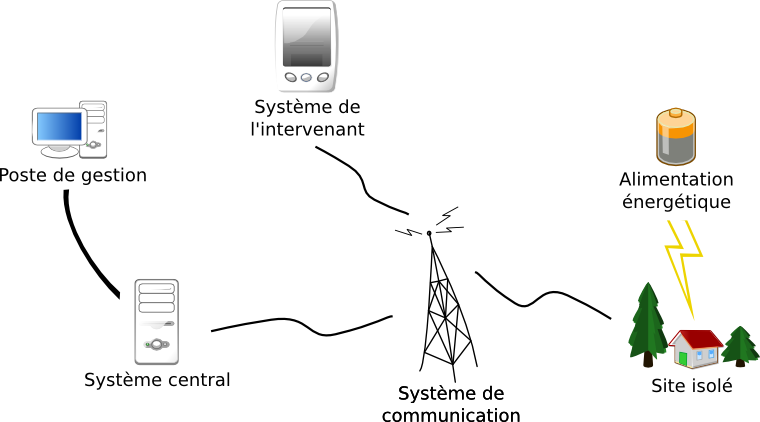
\includegraphics[width=.75\textwidth]{schema_architecture_generale.png}
\caption{Schéma de l'architecture générale de la solution}
\label{figure:schema_archi_generale}
\end{center}
\end{figure}

\end{document}
